\chapter{Discussion \& perspectives}
{\hypersetup{linkcolor=GREYDARK}\minitoc}

\section{Summary of main results}

Evolution of molecular sequences is seen as a stochastic process, where one component of this process is creating diversity through mutation, another antagonistic component is filtering out this diversity through selection, and finally the balance between these components is arbitrated by drift.
Applied to protein coding DNA sequences, this stochastic process results in a pattern of substitution along of species tree, where phylogenetic codon models captures intrinsic parameters of evolution.

Firstly, because the composition of protein coding DNA sequences does not reflect the underlying mutational process, but its filtering by selection at the level of amino-acids, a careful phenomenological modeling is necessary to uncover mutational process and nucleotide fixation bias.
Mutational bias result in fixation bias in the other direction.
By modeling fixation bias, mutational bias can be inferred reliably in the context of classical (i.e.\ non mechanistic) codon models.

Secondly, the balance between mutation and selection is arbitrated by drift, which is mediated by effective population size and its changes along a phylogeny can be estimated by mechanistic codon models.
It is possible to construct and implement mechanistic models of evolution parameterized by drift across branch and selection across sites.
There is persistent signal in substitution patterns that relates to past drift, and the variation of effective population size can be estimated.
However, assumptions on the properties of the fitness landscape, namely that each site is independent results in low response of $\omega$ to changes in $\Ne$.

Finally, selection for protein stability imply an analytical relationship between the rate of evolution and effective population size and protein expression level.


\section{Epistasis and entrenchment}

A blind spot of the mutation-selection phylogenetic codon models at least those explored here, is the assumption of site-independence.
This assumption is convenient, both computationally and statistically.
Computationally, each site is considered an independent Markov chain (markov process).
Statistically, model can rely on mixture models or penalized likelihood to estimate site-specific amino-acid fitness profiles
In contrast, from a modeling and inference perspective, accounting for epistasis is challenging  both in terms of parametrization and computational complexity~\citep{Rodrigue2005, Manhart2014}.
This complexity is the main reason why epistatis is generally ignored in phylogenetic models, and more particularly in codon models.

Empirically, however, many reasons to believe that this hypothesis of site-independence is not adequate, especially in the context of protein biophysics (see chapter \ref{chap:intro-physic-proteins}).
This approximation is problematic, and we can wonder what are the consequences of ignoring epistatis in the contexte of phylogenetic inference?
Pragmatically, how can we ultimately account for epistasis in inference?

Fundamentally, any model modeling fitness at the site level (without epistasis) implies a slow dynamic and a strong susceptibility, and adding epistasis to the model imply a faster dynamic and a weaker susceptibility.
Intuitively, this effect originates in the fact that each site has to adapt independently to changes in $\Ne$ leading to overall a slow response substitutions must affect all sites, and a strong susceptibility since each site will change its position in the fitness landscape.
Taking into account epistasis, the burden of adapting to changes in $\Ne$ is shared by more sites, such that all of them don't have to switch position.
This effect explains the low magnitude of $\Ne$ variation estimated with site-independent mechanistic codon models in chapter \ref{chap:MutSelDrift}.
Moreover, this translates with response of $\omega$ to changes in $\Ne$ in chapter \ref{chap:GenoPhenoFit}, because all sites of the sequences are involved in non-specific epistasis.
Susceptibility of $\dnds$ to changes in $\Ne$ is between two extremes, site independent fitness landscapes, and phenotype define for the whole sequence.
A remaining gap between quantitative predictions of biophysical models and empirical observations about response of omega to changes in $\Ne$ and expression level.

Mechanistically, accounting for epistasis can be 
Globally, the fitness landscape is fixed, but for a given site it appears as variable.
On the other hand, entrenchment due to specific epistasis has implication in terms of the assumption of a static fitness landscape.
Fitness landscapes are considered static, where the current sequence is sitting on the high ground of the fitness landscape, where by high ground I mean that the gap between peaks and current sequence is on the order of $1 / \Ne$.
With epistasis, fitness landscape is not static but dynamic, and for a specific site the proposed mutations are mostly from high ground into a fitness valley, where such valley is getting deeper and deeper with time.
In other words the selection coefficient of proposed mutations are getting increasingly negative with time, mimicking a dynamic fitness landscape.

As a result, statistical method relying on site-independent processes while accounting for other sites consist in obtaining the marginal process for a specific site, derived analytically from the joint process integrated over the other sites.
Projecting a joint process of several sites into a single site process leverages mean-field theory developed in statistical physics, and as been used to developed phylogenetic models accounting for protein structure \citep{Chi2018} and protein stability \citep{Arenas2015a, Arenas2017}.
Unfortunately, these methods are not parameterized directly in terms of parameters of evolution, namely mutation and effective population size, and the estimated fitness parameters can not be related to empirically determined parameters. 


\section{Adaptive landscape}
\label{sec:adaptative-landscape}

Another blind spot of the mutation-selection model is the assumption of a static fitness landscape.
The mutation-selection equilibrium under a fixed fitness landscape is essentially a nearly-neutral regime.
As a result, at equilibrium, sequence is close to optimum and therefore, most mutations are deleterious or compensate for previous deleterious mutations that got fixed.

This mutation-selection framework for detecting adaptation has been proposed relatively recently~\citep{Rodrigue2016}.
- still to be applied more broadly to empirical data, and compare it with classical codon models.


translates into a higher dN/dS than expected if the fitness landscape was fixed.
As a result, the assumption of static landscape can be turned into an advantage, where $\omega_0$ is the null model of absence of adaptive evolution,
$\omega$ and $\omega_0$ can be estimated along the sequence, such that mutation-selection framework can detect site-specific adaptive evolution in protein-coding genes.
Such method has been implemented in Bayescode, and the manuscript is available in appendix page~\pageref{sec-appendix:MutSelM3starMBE}.

- however, in its current form: assumes a constant $\Ne$ across the tree.
-this suggests to add $\omega_*$ (or $\omega_A$) in the mutsel-Ne
would potentially be more effective at detecting positive selection.
Also:  omega* could be allowed to vary across branches, like Ne.
This could have interesting applications:
For instance, do bats, compared to other mammals, have both stronger purifying selection (large Ne)
and stronger positive selection (larger omega*)?


Moreover, contrasting $\omega$ and $\omega_0$ lead to estimation of the rate of adaptive \gls{substitution} as:
\begin{align}
    \omega_A & = \omega - \omega_0 \\
    \omega_A & = \omega_* (1 - \omega_0)
\end{align}


Alternatively, proportion of adaptation estimated by phylogenetic codon models can be confronted to estimates of adaptation obtained with polymorphism dataset within species.
Originally pioneered by \citet{McDonald1991}, the ratio of non-synonymous over synonymous polymorphism ($\pnps$) supposedly solely contains non-adaptive polymorphism.
On the other hand, divergence data allows to estimate the ratio of non-synonymous over \glspl{synonymous} ($\dnds$), supposedly composed of a mixture of both advantageous \glspl{substitution} and non-adaptive (\gls{nearly-neutral}) \glspl{substitution}.
Thus the difference $\dnds - \pnps$ is the rate of adaptive evolution.
To note, the rate of non-adaptive evolution, $\pnps$ obtained with polymorphism data supposedly matches the compound parameters $\omega_0$ obtained uniquely from divergence data.
However, estimation of adaptive rate can be biased by moderately deleterious mutations~\citep{eyre-walker_quantifying_2002} and by the change in population size through time~\citep{eyre-walker_changing_2002}.
To overcome this biases, the method of \citet{Galtier2016} relies on the synonymous and non-synonymous site-frequency spectra (\acrshort{SFS}) to estimate the distribution of fitness effects of mutations (\acrshort{DFE}), modeled as a continuous distribution.
Subsequent development of these methods are reviewed in~\citep{Moutinho2019a}, intrinsically measuring the rate of non-adaptive evolution present in polymorphism data.

From the availability of divergence and polymorphism data, it is now possible to ask whether the rate of non-adaptive evolution measured by phylogenetic mutation-selection models matches the rate estimated from \acrshort{SFS}.
Are phylogenetic \gls{codon} models and population-genetics models independently estimating the same rate of adaption, and if not why is there a discrepancy should be understood.


\begin{figure}[H]
	\centering
	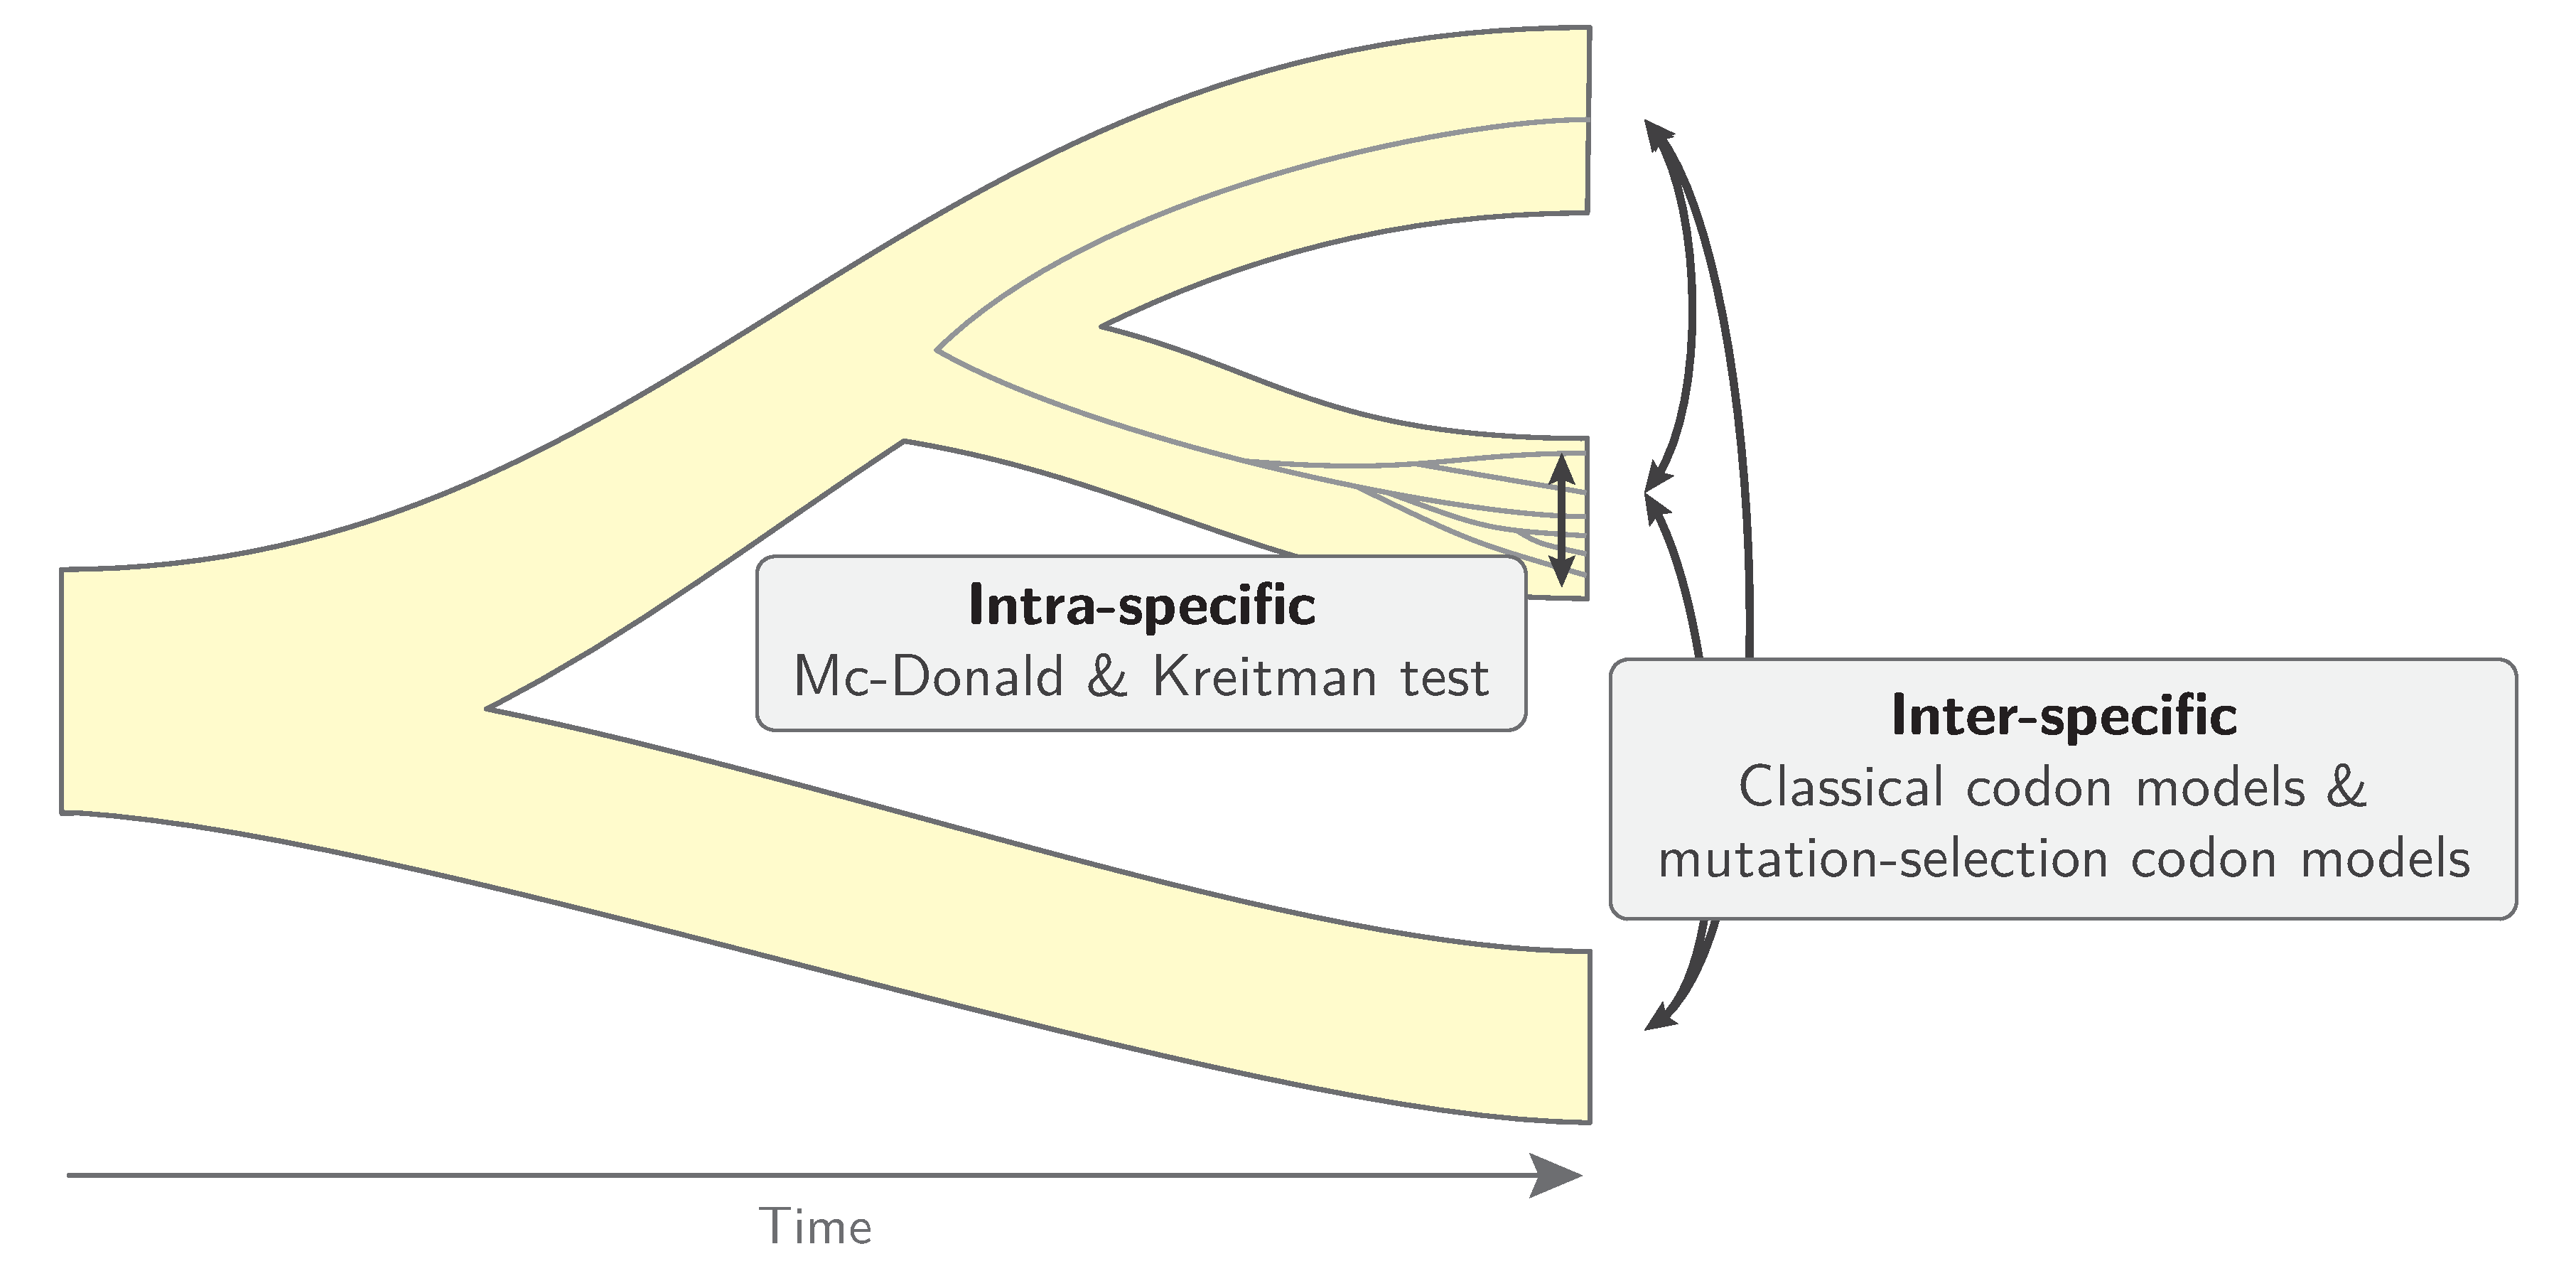
\includegraphics[width=\textwidth] {figures/inter-intra}
	\caption{Detecting adaptive evolution in coding sequences from inter- and intra-specific data}
\end{figure}


\section{Unifying phylogenetic and population-genetics model}
\label{sec:unifying-phylogenetic-and-population-genetics-model}

Along this manuscript, phylogenetic codon model has discarded diversity within species, and polymorphism has not been leveraged.
As a result, all divergence observed in the alignment are assumed to be substitutions, however some substitutions might be polymorphisms in the population but appear fixed in the sampled individuals.
Moreover, substitution are not instantaneous and ancestral shared polymorphisms can result in incomplete lineage sorting.
As a result, mistaking substitutions and polymorphisms is problematic since both are not sensitive to mutation, selection and drift in the same extent.
For example, number of polymorphisms increases with $\Ne$, while rate of neutral substitutions is insensitive to $\Ne$.
Also, mildly deleterious can be present in polymorphism while being filtered out by selection and not present in substitutions.
In contrast, mutational bias is entangled with selection in substitution, while being more easily detectable in polymorphism (\acrshort{SFS}).
Finally, polymorphism and divergence can be leveraged altogether to disentangle mutation, selection and drift.
As such we can wonder whether phylogenetic and population-genetics model can be unified?
% Charlesworth, D. (2010) Don’t forget the ancestral polymorphisms. Heredity, doi:10.1038/hdy.2010.14

Such integration between phylogenetic and population-genetics as been attempted in severals studies.
For example, \citet{Wilson2011} modeled codon evolution in a joint framework with $3$ species, allowing to analyze variation in selection pressures spatially along the genome and temporally between lineages.
This methodology proved to be computational intensive and scaled difficulty with the number of extant species.
Alternatively, modeling substitutions as mutational events followed by a gradual fixation allow to estimate nucleotide mutation rates and fixation biases from genetic variation within and between species, inherently accounting for shared ancestral polymorphisms and incomplete lineage sorting~\citep{DeMaio2013, Schrempf2016, Bergman2018, Schrempf2019}.
Hence, this methodology can be leveraged to disentangle gBGC and mutational bias~\citep{Borges2019, Borges2020}, although this methodology scale difficulty with the number of states of the models, and would be hard to translate from a nucleotide matrix (4 states) to a codon matrix (61 states).

Because mechanistic \gls{codon} models are based on population-genetics first principles, they can theoretically be extended to account for within species diversity.
The strategy can be to augment molecular divergence data between species with information about molecular polymorphism within species.
Such attempt has been tried during the first year of the PhD, where the formalism, based on Poisson Random fields can be found in appendices page \pageref{sec-appendix:PRF}.
The methods has found to be rather straightforward to implement into BayesCode, extending mutation-selection formalism.
First, it was found to be computationally intensive, even though optimizing the computation with sufficient statistics.
Secondly, the method provided sensible estimation of diversity ($\theta = 4 \Ne u$) based on generated simulation under Wright-Fisher model of evolution (SimuPoly).
However, the assumption of constant $\Ne$ along the phylogeny assumed by mutation-selection codon models was arguably the strongest assumption to relax in such context.
In other words, what sense would it make to integrate diversity in extant species that generally have quite different levels of diversity if $\Ne$ is considered constant along the phylogeny.
It was historically the reason to extend phylogenetic site-specific mutation-selection \gls{codon} models by incorporating branch-specific $\Ne$ presented in chapter \ref{chap:MutSelDrift}.
After extending mutation-selection with branch specific drift, we actually realized that the susceptibility of \gls{substitution} rate to changes in $\Ne$ is too strong because of site-independence assumption (chapter \ref{chap:GenoPhenoFit}), effectively amortizing the range of $\Ne$ which could be inferred.

Finally, even tough site- and branch-specific mutation-selection phylogenetic \gls{codon} models can be extended by incorporating signal of polymorphism, which actually has been implemented in Bayescode, I believe it is not yet the path forward to build an unified phylogenetic and population-genetics model.
Before being unified, I believe phylogenetic codon models and population-genetics method should be confronted, and the discrepancy should be understood, which is the path forward such that mean-fields models can be accommodated to population-genetics.

\section{Mechanistic and phenomenological models}
\label{sec:mechanistic-and-phenomenological-models}

% Categories of models
Models of inference are classified broadly into phenomenological and mechanistic~\citep{Rodrigue2010a}.
Mechanistic models dissect the causation chains and construct a model from first principles, while phenomenological models aims to determine the statistical significance of parameters.
Phenomenological models are for example the models parameterized directly in $\omega = dN/dS$, or by a fixed distribution of fitness effects.
They will for example tell us which branch of the tree, or which site of the sequence has a decrease or increase in $\omega$ but not the underlying reason for such changes, which can be either mutation, selection, drift or another evolutionary force.

% Site specific mechanistic models of evolution 
Contrarily, mechanistic models relate structural, population-genetics and ecological parameters to the \gls{likelihood} of the data.
As such, mechanistic inference models are suitable to construct an integrative framework relating the signal available in molecular sequences to structural parameters, expression level across genes and \gls{effective-population-size} across lineages.
Once such models is fitted to the data, the estimated parameters can be confronted to their independent empirical estimate, which allow to robustly test the model since orthogonal estimation of biological and ecological parameters should be congruent~\citep{Dasmeh2014}.
Additionally, once model robustness has been assessed, this inference framework could allow to estimate unknown variable, for example ancestral \gls{effective-population-size}, with enough signal and calibration of the other parameters. 


Altogether, I argue that our theoretical results are a building block to construct an integrated inference framework of molecular evolution, since such models are bridges between intrinsic biological parameters and the signal extractable from molecular sequences.
In order to reduce the complexity of mechanistic models, analytical models could allow to relate microscopic parameters of protein coding sequences to macroscopic parameters of evolution in a similar fashion of chapter \ref{chap:GenoPhenoFit}.
Subsequently, the microscopic parameters can be inferred from divergence and polymorphism data, and compared to their experimental estimation.

From chapter  \ref{chap:NucleotideBias}, I realized that mean-field models are useful tools to disentangle mutation and selection, such that depending on the site-specific landscape can be .
More parameter rich Bayesian framework can be parameterized directly in terms of mutation, selection and drift, however they are computationally intensive and simplifying assumption can trough the model off the ground \ref{chap:MutSelDrift}.
Finally, analytical models \ref{chap:GenoPhenoFit} can relate molecular parameters to parameters of evolution.
Altogether, these observations crystallized my opinion that mechanistically grounded models are necessary, but they should be complexified and simplified at the same time.
Complexified by incorporating for example site-dependence or polymorphism within species, and at the same time they should be simplified by means of analytical approximation, such for example using mean-fields models. 

\section{Reproducible science}
\label{sec:reproducible-science}

I argue that analytical models, computational simulations and inference models are complementary, but more importantly they are necessary to each others.
Theoretical modeling allow to understand the principles, simulations allow to verify the soundness.
Inference allow to extract and test the theoretical results using empirical data.
Simulations have a dual role, testing the robustness of both inference procedures and theoretical results, outside of their comfort zone and assumptions.
However, this assume we are confident enough to write reproducible computations, as such the next section is dedicated to my personal experience and take away.

First, I stand firmly on the ground that data, codes and scripts should be rendered open-access of any published and peer reviewed paper.
Practically, the availability of the data and source code should simply be enforced upon submission to journal, which is currently not the case for all journals, even in bio-informatics and genomics fields.
It is true that such enforcement bears the consequence to weight more burden on scientists upon publishing.
However, it avoids the bloating of technical debt, or research debt where we build on the ground of a dangerous and possibly shaky basement.
It encourages peer collaboration, both helping the team or person whom made the code available, and the community as a whole.
A straightforward way is to provide a \textit{git} versioned repository, with the advantage that collaboration is facilitated trough web hosted repository such as GitLab (hosted by institutions) or GitHub (hosted by Microsoft).

Nonetheless, code availability is a necessary condition, but not the sole requirement of reproducible research.
Specific instructions to reproduce the results should also be made available, where many tools are available to this aim~\citep{Wilson2014,Darriba2018}.
The first step necessary to reproduce a code is to have the required environment, meaning the necessary libraries and dependencies of the code and scripts.
For script and code written in Python, the package manager anaconda (or conda) provides a straightforward environment to configure the necessary libraries with their versions.
More complex environment requiring code compilation or system-level packages can leverage containerization technology such as Docker or Singularity for example, but any other containers implementing system-level virtualization is very helpful to provide the necessary libraries.
Once the environment is specified, the documentation can be made available as a README with the necessary instructions.
More generally, notebooks such as \textit{Jupyter Notebook}, \textit{RMarkdown} or \textit{org-mode} to name a few also provide an environment knitting together code and instructions, allowing to follow step-by-step experiments, analysis and results, in a similar fashion as laboratory notebook which are strictly required in wet labs.
It is important to note that notebooks can run code from a variety of languages (C++, Haskell, Java, Julia, Python, Wolfram Language, Matlab, Ruby, ...).
These tools are emerging in the community, as well as Workflow management system (Nexflow, Snakemake, etc) allowing to create reproducible and scalable data analyses running on computing clusters.

Using this range of tools helps other scientists which might want to understand, test or build upon published works.
Moreover, they are also very helpful for the person or team implementing them since a more rigorous and reproducible environment allows to more easily track down bugs and test programs under different conditions or dataset\footnote{Notebooks are very useful to present work and data analysis, but should not be used during development since they often offers poor integration with debugger and code inspection tools, enforce awkward software design patterns, and often result in bloated versioned repository.}.
During the development period, continuous integration pipelines are valuable to increase the reliability of code generation, which should be used whether working alone or inside team, but is of course more critical for collaborative code where one cannot control all the code written.
Collaborative coding practices such as peer-coding sessions is really useful to implement critical code at the core of the program under development.
I argue that the efficiency peer-coding sessions is provided by dividing the tasks into a group focused in the detailed implementation while the others a free to focus on edge cases and the overall implication of different implementations.
Moreover, peer-coding sessions provides a convenient and structured place for learning good practices, for expanding its technical knowledge while pruning bad habits.
An other remarkable practice is to write two independent version of the program, using if possible different algorithm and languages but with the same functionality, but most importantly by a different person.
Then testing the program against each others on the same conditions and dataset should result in the same outcome\footnote{An extreme version is adversarial coding (or chaos engineering), where the goal is to find conditions on which the adversary program fails.}.
Such model of reproducible computing experiment and analysis is laborious and demanding, but I argue this is the definition of reproducibility we collectively should aim for, namely where one can independently reproduce the same experiment, and if reproducibility fails one can run the code with different conditions to pinpoint the failing code (which might actually be in both versions).
Personally, having practiced this method I strongly believe it pervasively reduces our research debt that we might inadvertently burden other with whenever not realizing the program is bugged, and ultimately save us time on debugging and research conduction.
Finally, explaining to others our choices of algorithms, implementation and data structure requires us to express intelligibly our mental ideas and therefor better understand them, while gaining from others insight and algorithmic expertise.

\section{Concluding remarks}
\label{sec:concluding-remarks}

This work is modest attempt to construct integrated models of protein coding \acrshort{DNA} sequences evolution.
It succeeded in consolidating the idea that the patterns of \glspl{substitution} inform us on long term fluctuation of drift along branches, and selection along sites.
It did not succeeded in modeling the fitness landscape, apparently either too site-specific, or integrated over too many sites.
It is an indication that fitness landscape of protein coding sequences is between this two extremes.
It is building block to bridge phylogeny and population-genetics, constructing an integrated framework is theoretically possible but with limited scope.
However, confronting the estimation of phylogenetic \gls{codon} and population-genetics model, through for example the rate of adaptive \gls{substitution}, is a path forward in an integrated view of .
Finally, I believe this thesis is not providing any ground breaking, nor disruptive results, but instead is consolidating theoretical models on which molecular evolution is based, and points out the pitfall to avoid.
Science, alike a mutation-selection process not is optimized but as to trade off exploration of new ideas and exploitation of old ones.
Attempts to build bridges and connection between fields, alike \gls{recombination}, can bring the best of both worlds but many attempts are required.